\section{Introduction}
\begin{frame}{Theta-Curves}
	\begin{itemize}
		\item A \term{theta-curve} $T$ is a graph embedded in $S^3$,
		which consists of two vertices $v_1$, $v_2$
		and three edges $e_1$, $e_2$, $e_3$,
		such that each edge joins the vertices.
		\item A \term{constituent knot $T_{ij}$}, $1 \le i < j \le 3$, is a subgraph of $T$
		that consists of two vertices $v_1$, $v_2$ and two edges $e_i$, $e_j$.
		
		\item Theta-curves are roughly classified by comparing the triples of constituent knots.
		
		\item A theta-curve is said to be \term{trivial} if it can be embedded in a 2-sphere in $S^3$.

		$$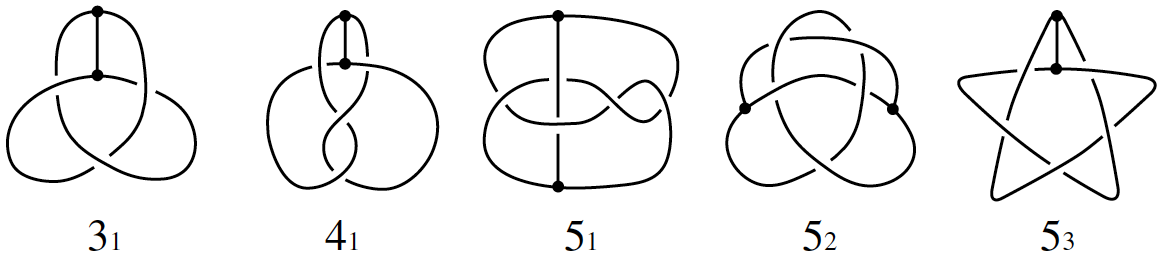
\includegraphics[width=.8\linewidth]{theta_exe.png}$$
	\end{itemize}
\end{frame}

\begin{frame}{Handcuff Graphs}
	\begin{itemize}
		\item \term{Handcuff graph} H is the graph which consists of two loops and an edge jointing the vertices of each loop.
		\item A \term{constituent link $H_{12}$}, is a subgraph of $H$
		that consists of two vertices $v_1$, $v_2$ and two edges $e_1$, $e_2$.

	\end{itemize}

	$$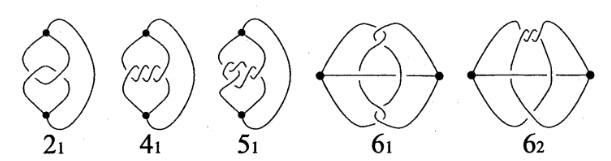
\includegraphics[width=.8\linewidth]{handcufflist.png}$$
\end{frame}

\begin{frame}{Reidemaister Moves for Theta-Curves and Handcuff Graphs}
	\medskip
	\begin{enumerate}
		\item[\mybf{I.}] \quad\raisebox{-15pt}{
\includegraphics[width=36pt,height=36pt]{y101}} \quad $\longleftrightarrow$ \quad \raisebox{-15pt}{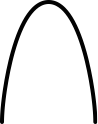
\includegraphics[width=36pt,height=36pt]{y103}} \quad $\longleftrightarrow$ \quad \raisebox{-15pt}{
\includegraphics[width=36pt,height=36pt]{y102}}\medskip
		\item[\mybf{II.}] \quad\raisebox{-15pt}{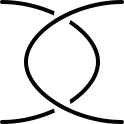
\includegraphics[width=36pt,height=36pt]{y111}} \quad $\longleftrightarrow$ \quad \raisebox{-15pt}{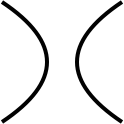
\includegraphics[width=36pt,height=36pt]{y93}} \quad $\longleftrightarrow$ \quad \raisebox{-15pt}{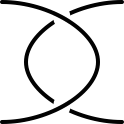
\includegraphics[width=36pt,height=36pt]{y112}}\medskip
		\item[\mybf{III.}] \quad\raisebox{-15pt}{
\includegraphics[width=36pt,height=36pt]{r31}} \quad $\longleftrightarrow$ \quad \raisebox{-15pt}{
\includegraphics[width=36pt,height=36pt]{r32}} \qquad\qquad\raisebox{-15pt}{
\includegraphics[width=36pt,height=36pt]{y121}} \quad $\longleftrightarrow$ \quad \raisebox{-15pt}{
\includegraphics[width=36pt,height=36pt]{y122}}\medskip
		\item[\mybf{IV.}] \quad\raisebox{-15pt}{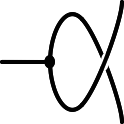
\includegraphics[width=36pt,height=36pt]{y141}} \quad $\longleftrightarrow$ \quad \raisebox{-15pt}{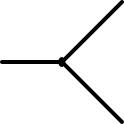
\includegraphics[width=36pt,height=36pt]{y143}} \quad $\longleftrightarrow$ \quad \raisebox{-15pt}{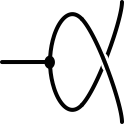
\includegraphics[width=36pt,height=36pt]{y142}}\medskip
		\item[\mybf{V.}] \quad\raisebox{-15pt}{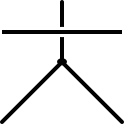
\includegraphics[width=36pt,height=36pt]{y131}} \quad $\longleftrightarrow$ \quad \raisebox{-15pt}{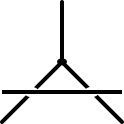
\includegraphics[width=36pt,height=36pt]{y132}} \qquad\qquad\raisebox{-15pt}{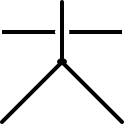
\includegraphics[width=36pt,height=36pt]{y133}} \quad $\longleftrightarrow$ \quad \raisebox{-15pt}{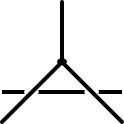
\includegraphics[width=36pt,height=36pt]{y134}}
	\end{enumerate}
\end{frame}

\begin{frame}{Arc Presentation}
    \begin{itemize}
        \item \term{Arc presentation} of a theta-curve or handcuff graph is an embedding of them.
        \item It is contained in the union of finitely many half planes (called \term{pages}).
        \item The embedding is with the common boundary line (called \term{axis}).
        \item Each vertex lies in the axis.
        \item Each page contains a properly embedded single arc.
        \item \term{Arc index}, is the minimal number of pages among all possible arc presentations of graph.
        \item This arc presentation with the minimal number of pages is \term{minimal arc presentation}.
    \end{itemize}
\end{frame}

\begin{frame}{Arc Presentation}
    \centering
    \begin{tabu}{X[c]X[c]X[c]}
        \raisebox{-1cm}{
\includegraphics[height=1cm]{Trefoilimage.png}} &
        \raisebox{-1cm}{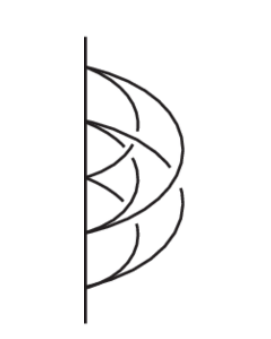
\includegraphics[height=1.75cm]{trefoil arc presentation.png}} &
        \raisebox{-1cm}{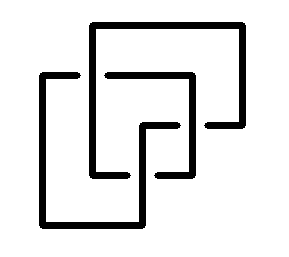
\includegraphics[height=1cm]{trefoil_grid.png}} \\
        Trefoil & Open Book & Grid Diagram
    \end{tabu}
    \centering
    \begin{tabu}{X[c]X[c]X[c]}
        \raisebox{-1cm}{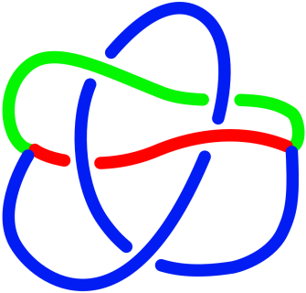
\includegraphics[height=1cm]{theta52.png}} &
        \raisebox{-1cm}{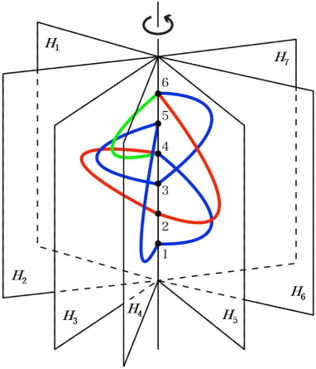
\includegraphics[height=1.75cm]{openbook.png}} &
        \raisebox{-1cm}{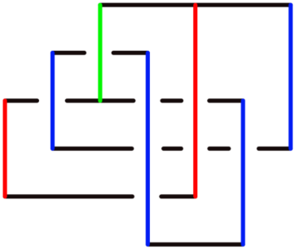
\includegraphics[height=1cm]{grid.png}} \\
        $\theta_{5,2}$ & Open Book & Grid Diagram
    \end{tabu}
    \centering
    \begin{tabu}{X[c]X[c]X[c]}
        \raisebox{-1cm}{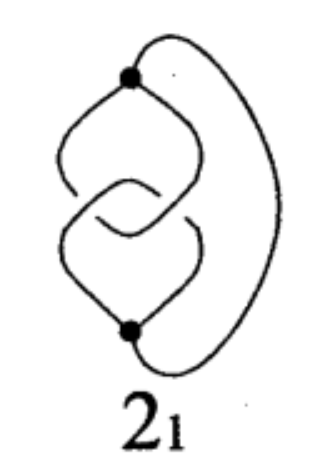
\includegraphics[height=2cm]{handcuff.png}} &
        \raisebox{-1cm}{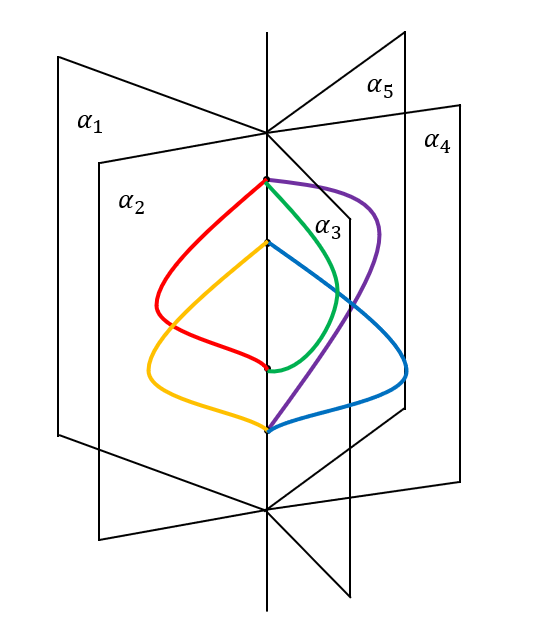
\includegraphics[height=1.75cm]{handcuff_openbook.png}} &
        \raisebox{-1cm}{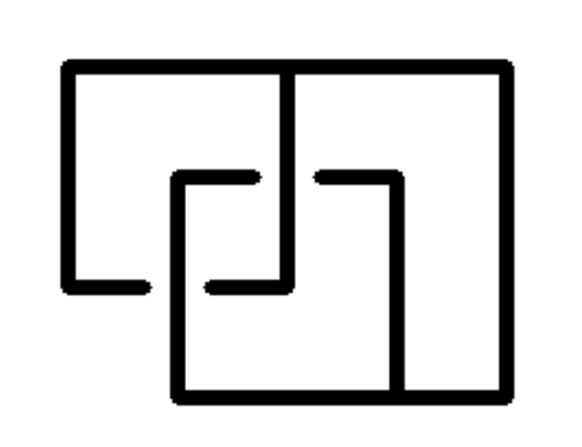
\includegraphics[height=1cm]{handcuff grid diagram.png}} \\
        $\Phi_{2,1}$ & Open Book & Grid Diagram
    \end{tabu}
\end{frame}


\begin{frame}{Grid Diagram}
	\begin{itemize}
        \item The \term{grid diagram} of theta-curve or handcuff graph is a diagram with only vertical strand and horizontal strands.
        \item (number of vertical strands) + 1 = (number of horizontal strands)
        \item At every crossing, the vertical strand crosses over the horizontal strand.
        \item No two horizontal strands are in the same row.
        \item No two vertical strands are in same column.
    \end{itemize}
\end{frame}

\begin{frame}{Grid Diagram}
    \begin{itemize}
        \item A grid diagram gives rise to an arc presentation and vice versa.
    \end{itemize}
    \centering
    \begin{tabu}{X[c]X[c]}
        \raisebox{-1cm}{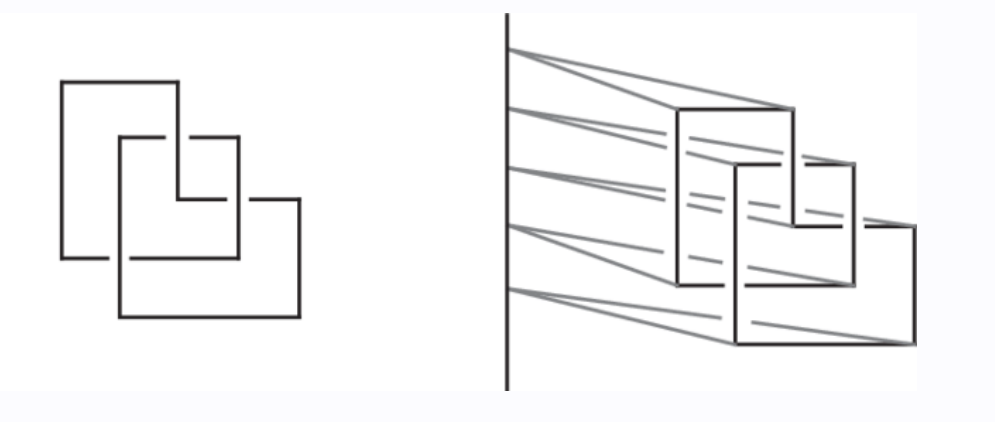
\includegraphics[height=4cm]{grid_diagram_1.png}} &
        \raisebox{-1cm}{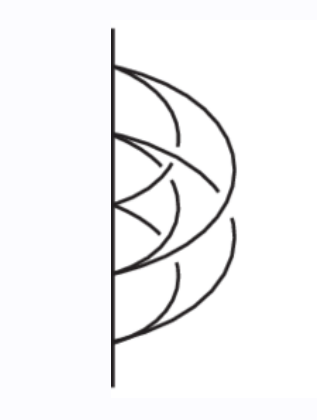
\includegraphics[height=4cm]{grid_diagram_2.png}} \\
    \end{tabu}
\end{frame}

\begin{frame}{Arc Presentation of the Theta-Curve and Handcuff Graph}
	\begin{thm}
    Every theta-curve and handcuff graph admit a grid diagram.
    \end{thm}
	\mypf
    \begin{center}
    \begin{tabu}{c c c}
        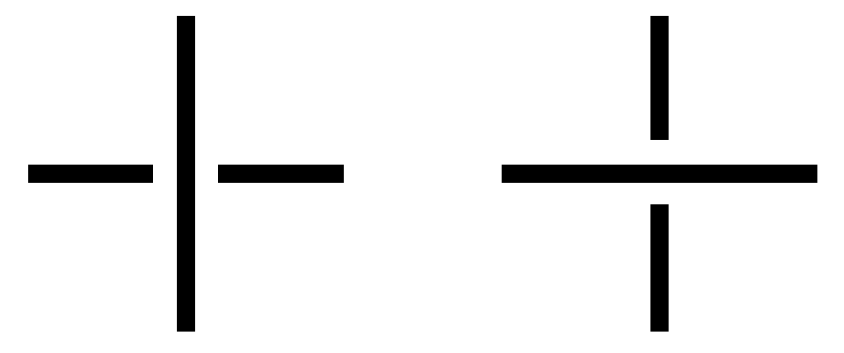
\includegraphics[width=0.2\linewidth]{figure/crossings.png} &
        \raisebox{0.5cm}{$\xmapsto{}$} &
        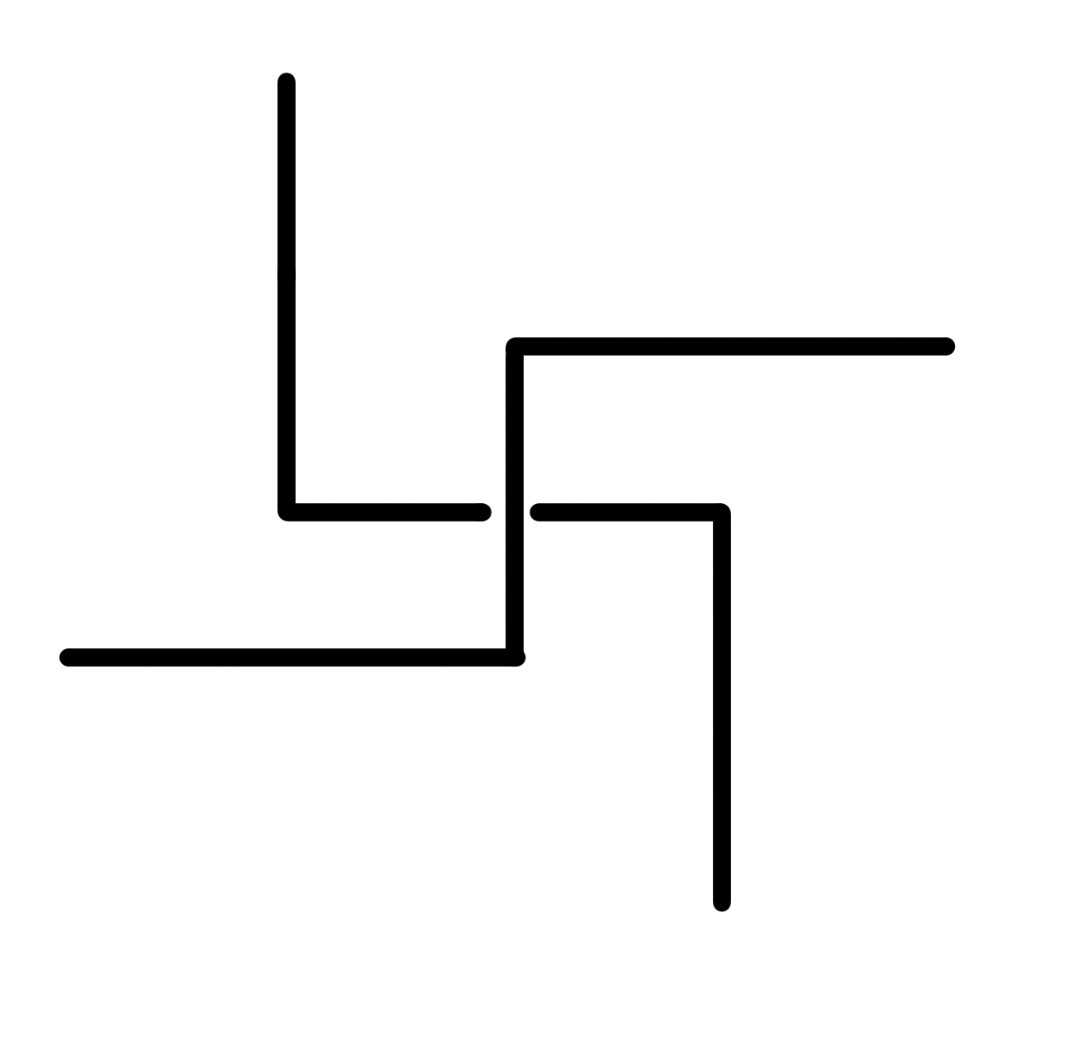
\includegraphics[width=0.1\linewidth]{changed_crossing.jpg}
    \end{tabu}
    \begin{tabu}{c}
        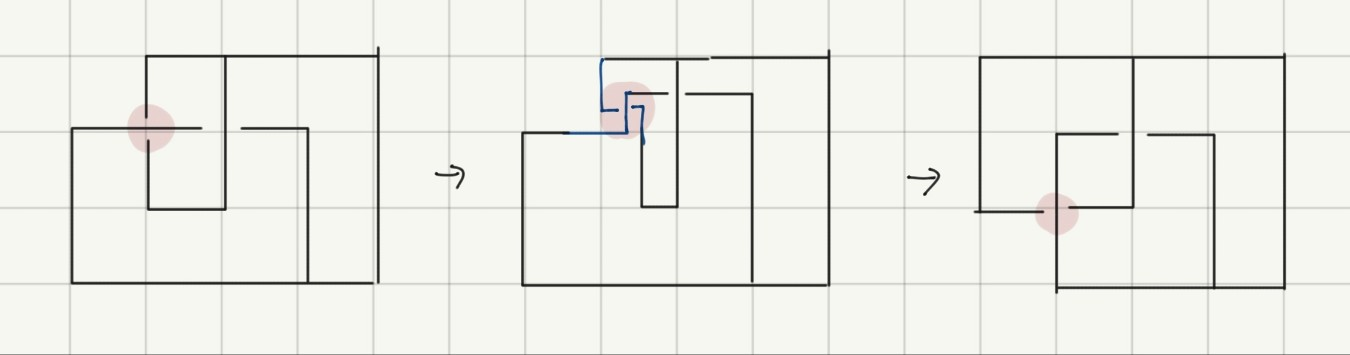
\includegraphics[width=0.5\linewidth]{crossing_change_example.jpg}
    \end{tabu}
    \end{center}
    \begin{corollary}
    Every theta-curve and handcuff graph admit a arc presentation.
    \end{corollary}
\end{frame}
